
\documentclass[11pt,a4paper]{article}

\usepackage[utf8]{inputenc}
\usepackage[T1]{fontenc}
\usepackage[spanish]{babel}

\usepackage{tgpagella}
\usepackage{geometry}
\usepackage{graphicx}
\usepackage{xcolor}
\usepackage{titlesec}
\usepackage{fancyhdr}
\usepackage[parfill]{parskip}
\usepackage[expansion=false]{microtype}
\usepackage{hyperref}
\usepackage{setspace}
\usepackage{needspace}

\geometry{top=3.0cm,bottom=3.0cm,left=3.5cm,right=3.5cm}

\setlength{\parskip}{0.65em}
\setlength{\parindent}{0em}

\definecolor{azulai}{RGB}{30,80,140}
\definecolor{doradoai}{RGB}{140,90,0}
\definecolor{grisai}{RGB}{70,70,70}

\titleformat{\section}
{\Large\bfseries\color{azulai}}
{}{0em}{}
[{\color{azulai}\titlerule[0.5pt]}]

\titlespacing*{\section}{0pt}{1.8em}{0.8em}

\titleformat{\subsection}
{\large\bfseries\color{doradoai}}
{}{0em}{}

\titlespacing*{\subsection}{0pt}{1.2em}{0.4em}

\pagestyle{fancy}
\fancyhf{}

\rhead{\textcolor{grisai}{\small Virginia Riezu — Arquitectura Interna}}
\lhead{\textcolor{grisai}{\small Carta Natal Base}}

\cfoot{\textcolor{grisai}{\small\thepage}}

\renewcommand{\headrulewidth}{0.3pt}

\hypersetup{
colorlinks=true,
linkcolor=azulai,
urlcolor=azulai
}

\setstretch{1.4}

\begin{document}

% ── PORTADA ──────────────────────────────────────────────────────────────

\begin{titlepage}

\centering

\vspace*{1.5cm}

{\Huge\bfseries\color{azulai} Carta Natal Base}\\[0.5cm]

{\large\color{grisai} Arquitectura Interna}\\[0.4cm]

{\small\itshape\color{grisai}
Un método para sostener cuerpo, energía y vida con coherencia
}\\[2cm]

{\huge\color{doradoai} Virginia Riezu}\\[1.5cm]

{\Large 06/09/1975 \quad 01:30}\\[0.3cm]

{\Large Pamplona, España}\\[0.3cm]

{\normalsize
Lat: 42.8157° \quad
Lon: -1.6522° \quad
UTC+02:00
}\\[0.5cm]

{\normalsize
Ascendente: Géminis 29°04'
}\\[2.5cm]

\vfill

{\small Generado el 20/05/2026}

\end{titlepage}


% ── INTRODUCCIÓN ─────────────────────────────────────────────────────────────

\section*{Introducción}

Esta carta natal base no busca definir quién eres.

La astrología se utiliza aquí como lenguaje de observación:
una forma de mirar cómo se organiza tu energía,
qué registros aparecen con más facilidad
y qué dinámicas pueden influir en tu manera de vivir, sostenerte y relacionarte con el entorno.

No se trata de una lectura predictiva ni de una identidad fija.
Es un mapa inicial de orientación.

Las siguientes páginas muestran únicamente las capas principales de la carta:
los ejes más visibles,
la distribución general de la energía
y algunos patrones básicos desde los que sueles moverte.

\vspace{0.4cm}

\newpage


% ── RUEDA ────────────────────────────────────────────────────────────────

\section{Carta Natal}

\begin{center}
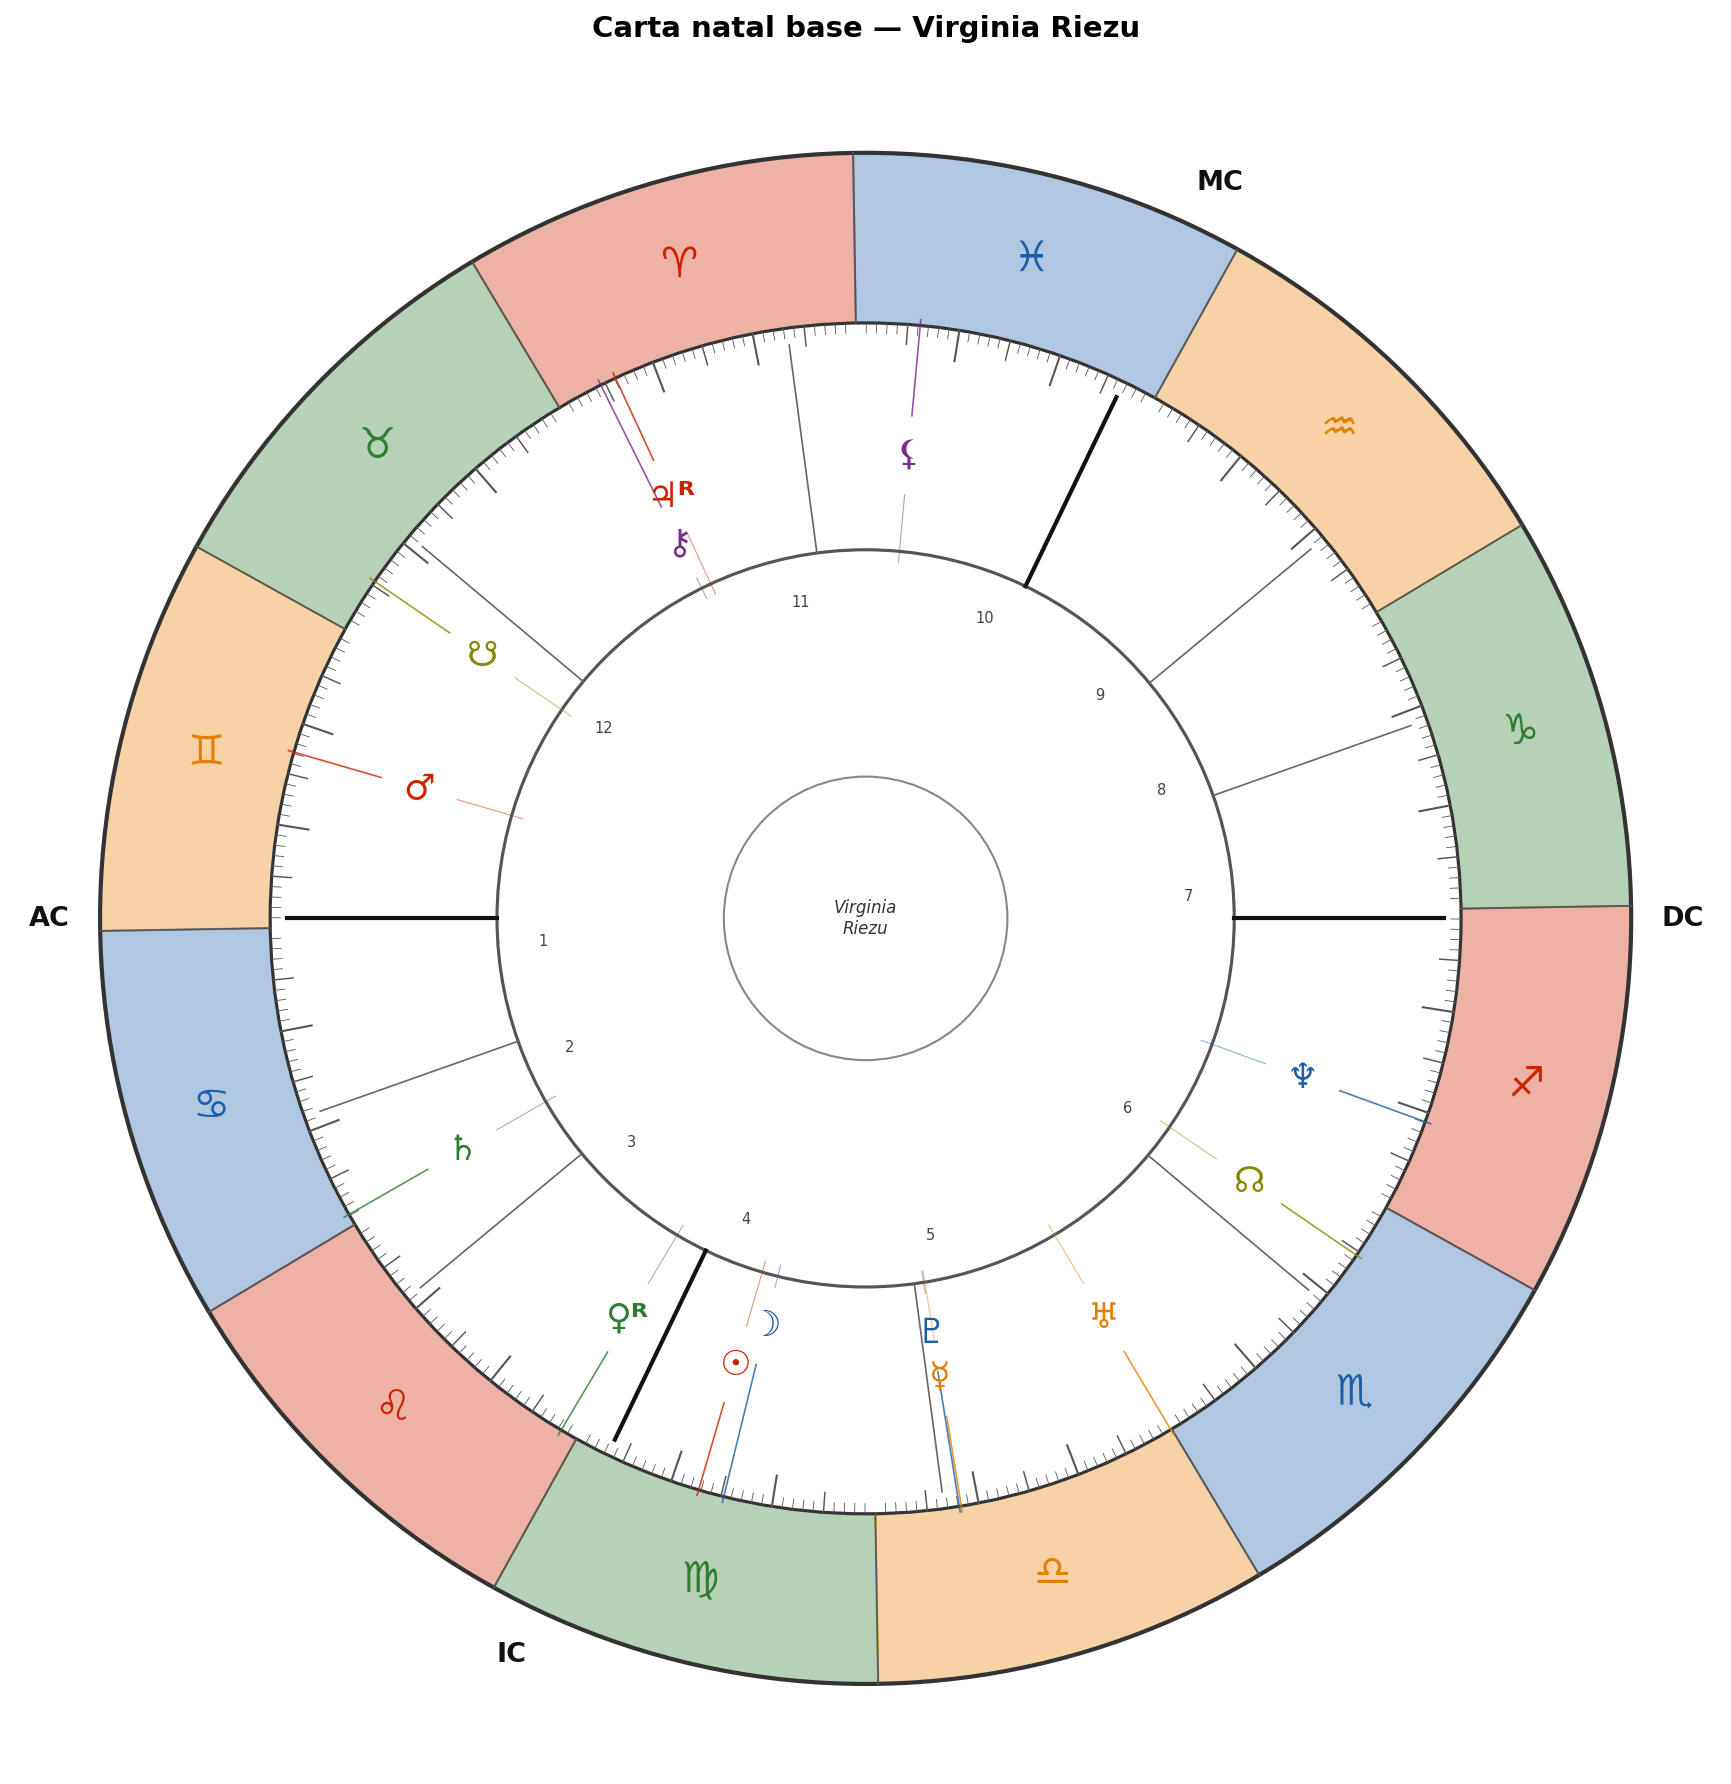
\includegraphics[width=0.8\textwidth]{Virginia_Riezu_carta_base_rueda.png}
\end{center}

\vspace{0.8cm}

% ── POSICIONES PRINCIPALES ───────────────────────────────────────────────

\section{Posiciones principales}

\begin{center}

Sol en Virgo — Casa 4\\
Luna en Virgo — Casa 4\\
Ascendente Géminis\\
Medio Cielo en Piscis

\end{center}

\vspace{0.5cm}

{\small\itshape
La lectura ampliada desarrolla el mapa completo de posiciones,
aspectos y configuraciones de la carta.
}

\vspace{0.8cm}
\Needspace{5\baselineskip}

% ── VISIÓN GENERAL ───────────────────────────────────────────────────────

\section{Visión general}

Tu carta muestra esta distribución de elementos: Fuego 3.5, Tierra 4, Aire 8, Agua 1. El elemento más presente es Aire (pensamiento, comunicación y necesidad de perspectiva). Esto señala un registro que suele aparecer con facilidad en tu forma de funcionar. El elemento menos presente es Agua (sensibilidad, percepción emocional y conexión con el entorno). No significa ausencia, sino una cualidad que puede necesitar más atención consciente. Tu Medio Cielo en Piscis orienta tu presencia pública hacia la sensibilidad, imaginación y capacidad de adaptación.

\vspace{0.8cm}
\Needspace{5\baselineskip}

% ── LOS TRES PILARES ────────────────────────────────────────────────────

\section{Los tres pilares}

\subsection{Sol en Virgo}

Con el Sol en Virgo, tiendes a orientarte hacia lo que puede mejorarse, ordenarse o hacerse de forma más precisa. Sueles fijarte en los detalles y buscar utilidad en lo que haces. Tu energía suele activarse cuando hay algo concreto que entender, organizar o resolver. Con el Sol en Casa 4, la intimidad, la sensación de hogar y la vida interior suelen tener mucho peso en tu desarrollo. Necesitas espacios donde puedas bajar la guardia y sentir cierta seguridad emocional. Muchas veces lo privado o lo emocional influye más en ti de lo que otras personas perciben desde fuera.

\vspace{0.8cm}
\Needspace{5\baselineskip}

\subsection{Luna en Virgo}

Con la Luna en Virgo, tiendes a observar y analizar bastante cómo te encuentras emocionalmente. El orden, la claridad y la sensación de que las cosas funcionan ayudan a que puedas sentirte más tranquilo. Muchas veces necesitas entender lo que ocurre para sentir estabilidad interna. Con la Luna en Casa 4, la intimidad, el hogar y la sensación de protección emocional suelen ocupar un lugar muy importante en tu vida. El entorno cercano influye bastante en cómo te sientes y en tu capacidad de descansar realmente.

\vspace{0.8cm}
\Needspace{5\baselineskip}

\subsection{Ascendente Géminis}

Con Ascendente en Géminis, sueles mostrarte de forma curiosa, comunicativa y mentalmente ágil. Tiendes a conectar rápido con el entorno a través de la conversación, las ideas o las preguntas. Las demás personas suelen percibir bastante movimiento y flexibilidad en tu forma de entrar en contacto.

\vspace{0.8cm}
\Needspace{5\baselineskip}

% ── CIERRE ───────────────────────────────────────────────────────────────

\section{Cierre}

Esta carta no busca definirte ni darte una identidad fija.

La astrología se utiliza aquí como lenguaje de observación:
una forma de mirar tendencias, ritmos y maneras de relacionarte con la vida.

La lectura ampliada desarrolla con más profundidad:
los vínculos,
la regulación emocional,
los patrones repetitivos,
la dirección de crecimiento,
las tensiones internas
y las configuraciones principales de la carta.

La lectura completa no busca darte más información.
Busca ayudarte a entender cómo sostener tu vida sin romperte por dentro.

\vspace{1cm}

\begin{center}

{\small\itshape\color{grisai}
Arquitectura Interna
}

\end{center}

\end{document}
